\begin{problem}
    Circle. $r = 6 \cdot \sin(\theta)$
\end{problem}

\begin{solution}
    To plot this by hand I find it important to really understand what's going on here. So, first things first, we can tell from the problem itself that we have a circle here. We can prove to ourselves why that is over the course of this problem. It's important to note that for this homework assignment I will be using digital plots, but I will attempt to showcase what's going on under the hood using a large amount of manual calculations. \medskip
    
    What I found works for me here it to start by sketching a sine/cosine wave representing our value of $r$. In this case we have a sine based sinusoid, so let's plot it! The amplitude for this guy will be 6, but otherwise it's a normal sine wave so we'll have a period of $2\pi$ and no phase shift.
    
    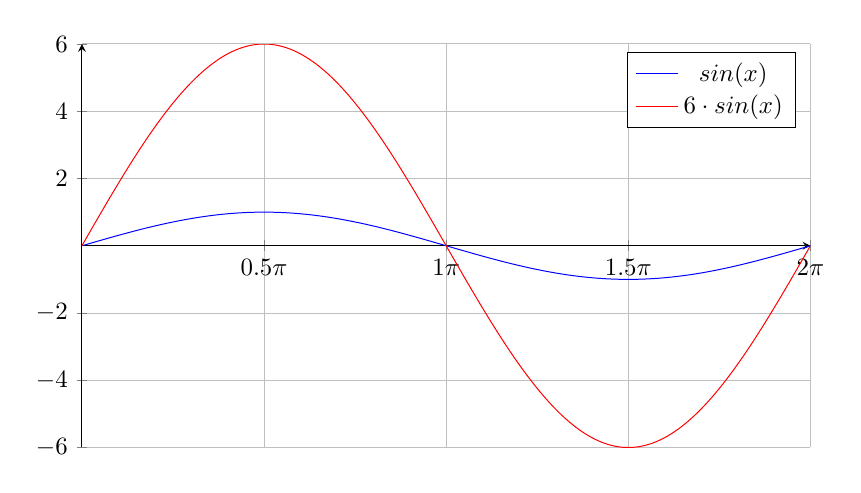
\begin{tikzpicture}[scale=0.9]
        \begin{axis}
            [
            grid=both,
            axis lines=middle,
            domain=0:2*pi,
            samples=200,
            no marks,
            xticklabels={-2$\pi$,-1.5$\pi$,...$\pi$,2$\pi$},
            xtick={-2*pi,-1.5*pi,...,2*pi},
            x post scale=1.5
            ]
            \addplot {sin(deg(x))};
            \addlegendentry{$sin(x)$};
            \addplot {6 * sin(deg(x))};
            \addlegendentry{$6 \cdot sin(x)$};
        \end{axis}
    \end{tikzpicture}
    
    From this we can glean some valuable information. $r$ is going to be 0 at $\theta = 0, 1\pi$ and $2\pi$. Also, that $-6$ is going to be important soon, keep an eye on it! Here's a quick table showing some values of r. 
    
    \begin{center}
    \begin{tabular}{|l|l|}
    \hline
    $f(\theta)$ & $r$ \\ \hline
    $f(0)$ & $0$ \\ \hline
    $f(\frac{\pi}{2})$ & 6 \\ \hline
    $f(\pi)$ & 0 \\ \hline
    $f(\frac{3\pi}{2})$ & -6 \\ \hline
    $f(2\pi)$ & 0 \\ \hline
    \end{tabular}
    \end{center}
    
    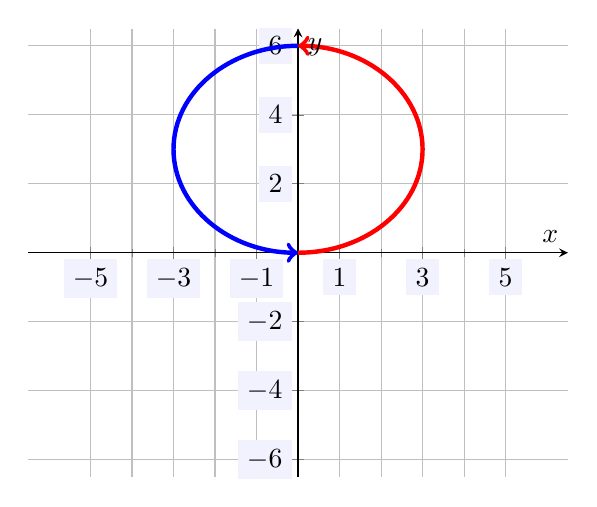
\begin{tikzpicture}[scale=1]
    \begin{axis}[grid=both,
    axis lines=middle,
    ticklabel style={fill=blue!5!white},
    xmin=-6.5,xmax=6.5,
    ymin=-6.5,ymax=6.5,
    xtick={-5,-3,-1,1,3,5},     
    ytick={-6,-4,-2,2,4,6},     
    minor tick = {-4,-2,...,4}, 
    xlabel=\(x\),ylabel=\(y\),
    samples=20]
    \draw[thick, dashed, black] (0, 3) circle (3);
    \draw[ultra thick, red, ->] (0,0) arc (-90:90:3) ;
    \draw[ultra thick, blue, ->] (0,6) arc (90:270:3);
    \end{axis}
    \end{tikzpicture}
    
    So, what's happening here is that we start with a radius of 0 which places us at the origin. At $\frac{\pi}{2}$ our radius goes up to 6. $\frac{\pi}{2}$ being, of course, straight up from the origin. We then cycle back to the origin when we hit $\theta = \pi$ thanks to our radius dropping back to 0. From there we go down to $\frac{3\pi}{2}$ which should be at the bottom of the y-axis, except our radius is negative so we flip right back up to the top of the y-axis again. The cycle continues forever. \medskip
\end{solution}